\subsection{Improved Open Traveling Salesman Ant Colony Optimization}
\label{subsec:aco}

The second layer of the framework solves the open traveling salesman problem on the cost matrix produced by the global planning layer. Given $N$ points consisting of a fixed start point $S$, $K$ intermediate goal points $\{T_1, \dots, T_K\}$, and a fixed end point $G$, the objective is to find the permutation of the $K$ goal points that minimizes the total path cost. On the basis of the ant colony optimization (ACO) metaheuristic, this paper introduces six integrated mechanisms: (1) a virtual-node method that converts the open traveling salesman problem into a standard closed traveling salesman problem; (2) Max--Min Ant System (MMAS) pheromone management with dynamically updated bounds; (3) an Ant Colony System (ACS) style pseudo-random proportional transition rule that balances exploration and exploitation; (4) Variable Neighborhood Descent (VND) local search accelerated by a $k$-nearest-neighbor candidate list; (5) a sigmoid progressive schedule that gradually shifts the search from exploration-dominated to exploitation-dominated; and (6) an adaptive stopping criterion.

\subsubsection{Virtual-Node Encoding of the Open Traveling Salesman Problem}
\label{subsec:virtual}

In the problem considered in this paper, the start point $S$ and the end point $G$ are distinct physical locations specified by the task (e.g., the origin and terminal stations of an autonomous bus), and they must be fixed at the two ends of every candidate solution; optimization is performed only on the ordering of the $K$ intermediate goal points. A naive encoding that treats all $N$ points as freely permutable produces invalid paths with misaligned endpoints, whereas a boundary-fixed encoding that pins the start and end points at the two ends of the path excludes them from the pheromone model and local search, thereby limiting the algorithm's ability to optimize the complete solution.

To this end, this paper adopts the virtual-node method to convert the open traveling salesman problem into a standard closed traveling salesman problem, a technique widely used in open vehicle routing problems~\textcolor{blue}{\cite{ref32}}. A virtual node $V = N + 1$ is introduced, and an extended cost matrix $\mathbf{D}_{\mathrm{ext}}$ of size $(N+1) \times (N+1)$ is constructed:
\begin{equation}
\mathbf{D}_{\mathrm{ext}}(i, j) =
\begin{cases}
0, & \{i, j\} = \{V, 1\} \\
0, & \{i, j\} = \{V, N\} \\
\mathrm{BIG}, & \begin{aligned}[t]
& (i = V \lor j = V) \land \\
& \{i, j\} \cap \{1, N\} = \varnothing
\end{aligned} \\
\mathbf{D}(i, j), & \text{otherwise}
\end{cases}
\label{eq:dext}
\end{equation}
where $\mathrm{BIG} = 2(N+1) \cdot \max_{i,j} \mathbf{D}(i,j)$ is a penalty value strictly larger than the cost of any feasible tour, ensuring that the virtual node is not directly connected to any intermediate goal point in any near-optimal tour. The zero-cost edges between the virtual node and the start and end points make the virtual node ``invisible'' to the path cost, whereas the penalty edges between the virtual node and the intermediate goal points force the virtual node to be adjacent only to the start and end points.

The ACO solver operates on the extended cost matrix $\mathbf{D}_{\mathrm{ext}}$ as a standard closed traveling salesman problem: all ants construct complete Hamiltonian tours over the $N+1$ nodes including the virtual node, and the pheromone matrix $\bm{\tau}$ covers the full $(N+1) \times (N+1)$ space. After the solver converges, the open-path visiting sequence is extracted from the optimal tour through the following steps:
\begin{enumerate}
\item Locate the virtual node $V$ in the tour.
\item Remove $V$ and read the remaining $N$ nodes in tour order.
\item Reverse the orientation if necessary so that the start point appears first and the end point appears last.
\end{enumerate}
The advantage of this transformation over the boundary-fixed encoding is that the start and end points fully participate in the pheromone model and local search, all standard closed traveling salesman operators apply uniformly, and cost evaluation reduces to a simple tour sum over $\mathbf{D}_{\mathrm{ext}}$ without separate boundary-cost terms.

The heuristic visibility matrix $\bm{\eta}$ is defined over the extended space. For node pairs involving the virtual node, the zero-cost edges from the virtual node to the start or end point are assigned a large heuristic value $\mathrm{BIG}$, which strongly attracts the virtual node to connect to its required neighbors; for all other pairs, the heuristic value is the reciprocal of the extended cost:
\begin{equation}
\eta_{ij} =
\begin{cases}
\mathrm{BIG}, & \{i, j\} = \{V, 1\} \text{ or } \{V, N\} \\
\dfrac{1}{\mathbf{D}_{\mathrm{ext}}(i,j)}, & \mathbf{D}_{\mathrm{ext}}(i,j) > 0 \\
0, & \text{otherwise}
\end{cases}
\label{eq:eta}
\end{equation}
The cost of a closed tour $\bm{\sigma} = (\sigma_1, \sigma_2, \dots, \sigma_{N+1})$ is the sum of the costs of all edges on the tour, including the closing edge $\sigma_{N+1} \to \sigma_1$.

\subsubsection{Max--Min Ant System Pheromone Update with Dynamic Bounds}

The Max--Min Ant System (MMAS)~\textcolor{blue}{\cite{ref23}} restricts pheromone values to an explicit interval $[\tau_{\min}, \tau_{\max}]$ to prevent unilateral domination and extinction, and concentrates deposition on elite solutions. This paper adopts this mechanism and specifies a bound-initialization and update procedure matched to the cost scale.

Accordingly, at each iteration all pheromone values are first evaporated as $\tau_{ij} \leftarrow (1 - \rho) \cdot \tau_{ij}$, where $\rho$ is the evaporation rate. After evaporation, pheromone is deposited at two solution levels: the edges of the iteration-best tour $\bm{\sigma}_{\mathrm{iter-best}}$ and the global-best tour $\bm{\sigma}_{\mathrm{global-best}}$ receive
\begin{equation}
\tau_{ij} \leftarrow \tau_{ij} + \frac{Q}{C_{\mathrm{iter}}}, \qquad
\tau_{ij} \leftarrow \tau_{ij} + \frac{Q}{C_{\mathrm{global}}}
\label{eq:deposit}
\end{equation}
respectively, where $Q$ is the deposition constant and $C$ is the corresponding tour cost. The deposit amount is inversely proportional to the tour cost, so shorter tours deposit stronger pheromone. Both deposition levels are applied simultaneously to the symmetric pair $(j, i)$, preserving an undirected pheromone model.

After deposition, all pheromone values are clamped to the interval $[\tau_{\min}, \tau_{\max}]$, whose bounds are dynamically updated according to the current global-best tour:
\begin{equation}
\tau_{\max} = \frac{1}{\rho \cdot C_{\mathrm{global}}}, \qquad
\tau_{\min} = \frac{\tau_{\max}}{N+1}
\label{eq:taumax}
\end{equation}
The initial pheromone matrix is set to a uniform value $\tau_0$, representing a neutral prior before search experience accumulates. At initialization the bounds are taken as $\tau_{\max}^{0} = 1/(\rho \cdot \tau_0 \cdot (N+1))$ and $\tau_{\min}^{0} = \tau_{\max}^{0}/(5(N+1))$, so that the initial value $\tau_0$ is not clipped during the early stage. Within each iteration the pheromone is updated in the following order: first evaporate, then deposit on the iteration-best and global-best tours according to Eq.~\textcolor{blue}{\eqref{eq:deposit}}, then clamp all pheromone values to the current $[\tau_{\min}, \tau_{\max}]$ interval, and finally recompute the bounds from the current global-best cost according to Eq.~\textcolor{blue}{\eqref{eq:taumax}}. A hard lower limit $\tau_{\min} \geq 10^{-6}$ is additionally imposed on the bounds to prevent pheromone on low-frequency edges from underflowing to zero and becoming completely extinct under small-scale costs. Dynamic bound updates are critical: as the search discovers better tours, the decrease in $C_{\mathrm{global}}$ increases $\tau_{\max}$, allowing the algorithm to express stronger confidence in its current best solution. Conversely, the ratio $\tau_{\min}/\tau_{\max} = 1/(N+1)$ maintains a constant relative gap between the minimum and maximum pheromone, preserving a baseline exploration probability for every edge regardless of the absolute scale. Regarding the matching of parameter magnitudes, the ratio of the deposit amount $Q/C$ to $\tau_{\max} = 1/(\rho C)$ equals $\rho Q$, which is approximately $56$ in the present implementation. Consequently, deposits on the edges of the best tour are typically truncated by $\tau_{\max}$ during the subsequent clamping; the effective reinforcement intensity is calibrated by $\tau_{\max}$, and $Q$ primarily affects the relative ordering of the per-edge deposits before clamping.

\subsubsection{Pseudo-Random Transition Rule in the Ant Colony System Style}

The pseudo-random proportional rule of the Ant Colony System (ACS)~\textcolor{blue}{\cite{ref22}} greedily selects the best candidate with a controllable probability and explores by roulette selection otherwise, balancing convergence and diversity. This paper adopts this rule as the transition mechanism during the path-construction phase.

In the concrete implementation, when an ant at the current node $u$ selects the next node from the set of unvisited candidates $\mathcal{U}$, it first computes the score of each candidate as $\mathrm{score}(v) = (\tau_{uv})^{\alpha} \cdot (\eta_{uv})^{\beta}$, where $\alpha$ and $\beta$ are the pheromone and heuristic weight exponents, respectively. The transition decision follows
\begin{equation}
v_{\mathrm{next}} =
\begin{cases}
\arg\max_{v \in \mathcal{U}} \; \mathrm{score}(v), & \text{with probability } q_0 \\
\mathrm{roulette}(\mathcal{U}, \mathrm{score}), & \text{with probability } 1 - q_0
\end{cases}
\label{eq:trans}
\end{equation}
where $q_0$ is the exploitation probability. In the exploitation case, the ant deterministically selects the highest-scoring candidate, equivalent to a greedy optimal step. In the exploration case, the ant performs roulette selection, in which each candidate $v$ is chosen with probability $\mathrm{score}(v) / \sum_{u \in \mathcal{U}} \mathrm{score}(u)$. If all scores are zero, i.e., all remaining nodes are unreachable, an unvisited candidate is selected at random as a fallback.

As can be seen, a larger $q_0$ causes more construction steps to adopt greedy selection and thus accelerates convergence, whereas a smaller $q_0$ increases the proportion of random exploration. Pairwise distances in the obstacle-constrained cost matrix typically exhibit spatial locality, so the heuristic $\bm{\eta}$ provides fairly reliable guidance; this makes a moderately high greedy probability beneficial for convergence while still preserving diversity.

\subsubsection{Variable Neighborhood Descent Local Search with Candidate-List Acceleration}
\label{subsec:vnd}

Although the paths constructed by ants are guided by pheromone and heuristic information, they are not necessarily locally optimal. A natural improvement is to apply local search to the current best solution at each generation, further refining solution quality by systematically examining neighboring permutations. Variable Neighborhood Descent (VND)~\textcolor{blue}{\cite{ref24}} is precisely such a class of methods: it invokes multiple neighborhood structures in sequence, each corresponding to a class of path transformations, and switches to the next structure when the current one can no longer improve the solution, until no neighborhood yields a better solution. Existing studies have shown that hybridizing MMAS or ACS with VND is highly effective for vehicle routing problems~\textcolor{blue}{\cite{ref25}}. However, standard VND must examine $O(K^2)$ neighborhoods for each operator, and the computational cost rises rapidly as the number of goal points grows, becoming a major bottleneck. Further observation reveals that many of these examinations are fruitless: when a pair of distant nodes participates in a 2-opt exchange, it rarely yields an improvement in tour cost.

To address this issue, this paper implements VND on the closed tour formed by the $N+1$ nodes including the virtual node, and alternates three neighborhood operators in a fixed order. The role of each operator and its associated candidate-list pruning condition are as follows:
\begin{enumerate}
\item \textbf{2-opt}: reverse a contiguous subsequence of the path as a whole, i.e., replace the original edges $(u, u^{+})$ and $(v, v^{+})$ with the edges $(u, v)$ and $(u^{+}, v^{+})$, thereby eliminating the path crossings common under Euclidean-type costs. Before evaluating this reversal, the cost change is computed only if at least one of the new edges $(u, v)$ and $(u^{+}, v^{+})$ belongs to the candidate-neighbor set.
\item \textbf{Relocate}: extract a node from its current position and insert it at another position in the tour, shifting the intermediate nodes accordingly; this is used to correct cases in which a node has been placed into the wrong path segment. Before evaluating the insertion, the examination proceeds only if the moved node $v$ and one of its new neighbors ($p$ or $p^{+}$) are mutual candidate neighbors.
\item \textbf{Swap}: exchange the positions of two nodes while keeping all other nodes unchanged; this applies when two nodes happen to be assigned to each other's better positions. Before evaluating the exchange, execution is considered only if the two nodes $a$ and $b$ to be swapped are mutual candidate neighbors.
\end{enumerate}
Within the VND loop, the above operators follow a \emph{first-improvement} strategy: 2-opt is applied repeatedly until the cost can no longer be reduced; if no further improvement is found, the search switches to relocate, and finally attempts swap. Whenever any operator produces an improvement, the next round restarts from 2-opt; the local search terminates when none of the three operators can improve the solution further.

In terms of computational efficiency, this paper introduces a precomputed candidate list to filter out clearly unpromising cases in the above evaluations, an idea widely used in local search for the traveling salesman problem~\textcolor{blue}{\cite{ref26}}. Specifically, for every node in the extended problem (a total of $N+1$), its $k$ nearest neighbors are preselected according to the extended cost matrix $\mathbf{D}_{\mathrm{ext}}$ and stored in a Boolean matrix $\mathbf{C}$, where $\mathbf{C}(i,j)=\mathrm{true}$ indicates that node $j$ is a candidate neighbor of node $i$; the term ``candidate neighbor'' used in the operators above always refers to nodes in this list. It should be noted that the pruning described above is deliberately conservative: an evaluation is skipped only when none of the new edges involved in a move belongs to the candidate-neighbor set. Such cases usually indicate that the move is unlikely to improve the tour, but this cannot be regarded as an absolute guarantee. The candidate-list size $k$ should be kept small, which both filters out a large amount of fruitless computation and retains the local structures most likely to yield improvements; when the extended cost matrix exhibits strong spatial clustering, improving edge exchanges occur almost exclusively between nearby nodes, making this setting particularly effective.

From a complexity perspective, without pruning each VND operator would need to examine $O((N+1)^2)$ candidate moves; with the candidate list, each node participates in only about $O(k)$ neighborhood checks, reducing the per-operator complexity to $O((N+1)\cdot k)$. When $k$ is on the order of single digits, the computational cost is reduced by approximately one order of magnitude relative to full-neighborhood examination; as $N$ grows, the acceleration becomes even more pronounced.

Algorithm~\textcolor{blue}{\ref{alg:vnd}} gives the complete pseudocode of candidate-list-accelerated VND. As a supplement, the three neighborhood operators above all follow the first-improvement principle, i.e., a move that reduces the tour cost is accepted and returned immediately once discovered; because the problem is defined on a closed tour, when a swap operation involves the first and last adjacent nodes of the tour, the wrap-around adjacency must also be taken into account, and the adjacency test under a linear path cannot be applied directly. The complete flow of the VND neighborhood search is shown in Fig.~\textcolor{blue}{\ref{fig:vnd_flow}}.

\begin{algorithm}[!t]
\caption{Candidate-list-accelerated variable neighborhood descent}
\label{alg:vnd}
\begin{spacing}{0.9}
\begin{algorithmic}[1]
\REQUIRE closed tour $\bm{\sigma} = [\sigma_1, \dots, \sigma_{N+1}]$, extended cost matrix $\mathbf{D}_{\mathrm{ext}}$, candidate boolean matrix $\mathbf{C}$
\ENSURE improved tour $\bm{\sigma}$ and its cost
\STATE $\mathrm{cost} \gets$ the cost of tour $\bm{\sigma}$ under $\mathbf{D}_{\mathrm{ext}}$;
\REPEAT
\STATE $\mathrm{improved} \gets$ false;
\STATE $[\bm{\sigma}, \mathrm{cost}, \mathrm{ok}] \gets$ apply the 2-opt operator with candidate-list pruning (first-improvement);
\STATE $\mathrm{improved} \gets \mathrm{improved}$ or ok;
\STATE $[\bm{\sigma}, \mathrm{cost}, \mathrm{ok}] \gets$ apply the relocate operator with candidate-list pruning;
\STATE $\mathrm{improved} \gets \mathrm{improved}$ or ok;
\STATE $[\bm{\sigma}, \mathrm{cost}, \mathrm{ok}] \gets$ apply the swap operator with candidate-list pruning;
\STATE $\mathrm{improved} \gets \mathrm{improved}$ or ok;
\UNTIL{$\mathrm{improved} = \mathrm{false}$}
\STATE $\mathrm{cost} \gets$ the exact cost of the final tour $\bm{\sigma}$;
\RETURN $\bm{\sigma}$, $\mathrm{cost}$;
\end{algorithmic}
\end{spacing}
\end{algorithm}

\begin{figure}[!t]
\centering
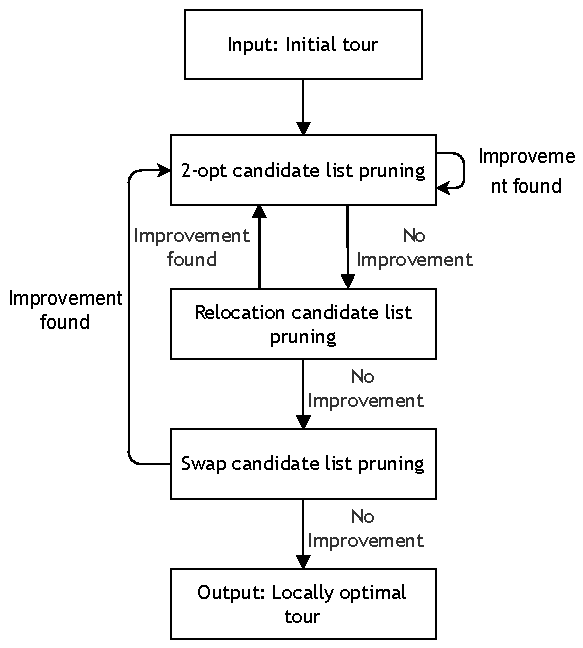
\includegraphics[width=3in]{figures/fig03_vnd_flow.pdf}
\caption{Flowchart of the VND neighborhood search sequence.}
\label{fig:vnd_flow}
\end{figure}

\subsubsection{Sigmoid Progressive Local-Search Scheduling}
\label{subsec:sigmoid}

Even with candidate-list acceleration, VND local search still requires considerable computation time. If local search were applied to every ant in every generation, resources in early iterations would often be wasted: at that stage the population has not yet identified promising regions of the search space, and refining low-quality paths yields limited benefit. In contrast, in the later stage, when pheromone has concentrated on high-quality regions, intensive local search becomes crucial for further polishing the solution. Clearly, applying local search to a fixed proportion of ants throughout the run is not ideal---a low proportion slows convergence, whereas a high proportion wastes computation on immature solutions. To this end, this paper dynamically adjusts the proportion of ants that receive VND local search during the iterations according to a sigmoid function:
\begin{equation}
\mathrm{optRatio}(t) = y_{\min} + (y_{\max} - y_{\min}) \cdot \frac{t^{a}}{t^{a} + (1 - t)^{a}}
\label{eq:sigmoid}
\end{equation}
where $t = (\mathrm{iter} - x_L) / (x_R - x_L)$ is the normalized position of the current iteration within the transition interval $[x_L, x_R]$; $y_{\min}$ and $y_{\max}$ are the lower and upper bounds on the proportion of ants that receive local search in the early and late stages of the search, respectively, and $a$ controls the steepness of the sigmoid curve. When $t$ is below $x_L$, $\mathrm{optRatio}$ equals $y_{\min}$; after $x_R$ it remains at $y_{\max}$; within the interval, the proportion transitions smoothly along the sigmoid curve.

This schedule smoothly shifts the search from broad exploration in the early stage (with low local-search overhead) to intensive refinement of high-quality solutions in the late stage, while a subset of ants maintains construction diversity. The relatively short transition interval $[0, 30]$ is chosen so that the proportion reaches its upper bound early; experiments show that the basic pheromone structure typically forms within about 30 generations. The sigmoid curve of $\mathrm{optRatio}(t)$ is shown in Fig.~\textcolor{blue}{\ref{fig:sigmoid}}.

After determining the number of ants that will receive local search in the current round as $n_{\mathrm{opt}} = \lceil n_{\mathrm{ants}} \cdot \mathrm{optRatio} \rceil$, the specific individuals must still be selected. This paper adopts a hybrid elite--random strategy: the top-ranked $n_{\mathrm{elite}} = \lceil n_{\mathrm{opt}} \cdot r_{\mathrm{elite}} \rceil$ elite individuals receive optimization first, strengthening the fine-grained polishing of high-quality solutions; the remaining $n_{\mathrm{random}} = n_{\mathrm{opt}} - n_{\mathrm{elite}}$ ants are drawn at random from the non-elite individuals and likewise receive optimization, creating opportunities to discover promising regions beyond the elites and maintaining a balance between exploitation and exploration. Here $r_{\mathrm{elite}}$ is the elite-ratio parameter.

\begin{figure}[!t]
\centering
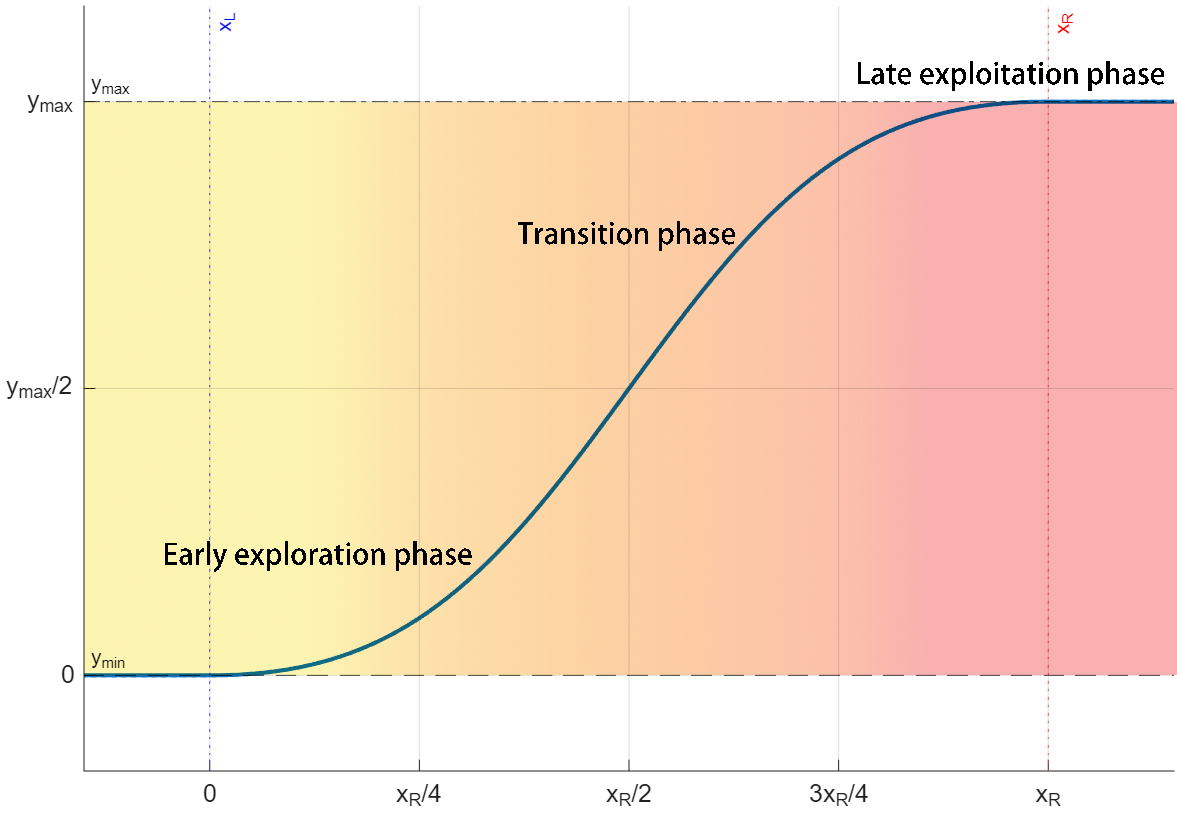
\includegraphics[width=2.5in]{figures/fig04_sigmoid}
\caption{Sigmoid curve of $\mathrm{optRatio}(t)$ as a function of the iteration number.}
\label{fig:sigmoid}
\end{figure}

\subsubsection{Adaptive Stopping Criterion}

The algorithm treats the maximum number of iterations $n_{\mathrm{iter}}$ as an upper bound on the iteration budget, to avoid failure to converge on difficult instances owing to insufficient budget. On easy instances, however, the population often converges long before this limit; further iterations only increase computational cost without improving solution quality. Conversely, stopping too early may miss better solutions. The stopping criterion must therefore distinguish between ``fully converged'' and ``temporarily not yet improved'', identifying true convergence while avoiding premature termination due to brief stagnation.

Specifically, the algorithm monitors two complementary indicators.

The first indicator is population homogeneity. When the ant colony converges to a narrow region of the search space, the tour costs produced by different ants become close to one another and the variance decreases accordingly. This paper characterizes it using the coefficient of variation (CV$= \sigma_{\mathrm{costs}} / \mu_{\mathrm{costs}}$, i.e., the ratio of the standard deviation to the mean) of the tour costs of the ants in each generation. When $\mathrm{CV}$ falls below a preset threshold $\varepsilon_{\mathrm{CV}}$, the population is considered to have become homogeneous---the tours are of roughly equal quality---and the probability of discovering new solutions through further search is already very low.

The second indicator is whether the best solution has entered stagnation. Even if some diversity remains within the population, the current global-best tour may linger near a local optimum for a long time. The algorithm therefore records the number of consecutive iterations in which the global-best cost has not improved; once this count reaches the preset limit $\mathrm{stagn}_{\max}$, the search is terminated.

To reduce the risk of premature stopping, the two criteria above are enabled only after a minimum number of iterations $\mathrm{minIter}$ has been completed. This is because in the early stage of the search the cost variance is usually large and the global best is still improving rapidly; monitoring convergence at that point can easily misclassify normal fluctuations as convergence. After a minimum amount of search, the pheromone structure has taken shape, and the stopping decision becomes more reliable.

\subsubsection{Integration Summary}

Combining the above designs, the MMAS-VND-CL algorithm organizes the six mechanisms into a single iterative search procedure: the extended cost matrix $\mathbf{D}_{\mathrm{ext}}$ is defined over the $N+1$ nodes including the virtual node, and both the pheromone model and local search operate in this space. The main steps of a single iteration are as follows:
\begin{enumerate}
\item Determine the proportion of ants that will receive local search in this round from the sigmoid curve.
\item All ants independently construct a Hamiltonian tour covering the $N+1$ nodes according to the ACS-style pseudo-random transition rule.
\item Select a subset of ants by the elite--random hybrid strategy and apply candidate-list-accelerated VND local search to their tours.
\item Update the current global-best tour and apply the adaptive stopping criterion to decide whether to terminate.
\item If the search continues, evaporate the pheromone, deposit it on the iteration-best and global-best tours, and finally apply dynamic clamping to the pheromone values according to the MMAS rules.
\end{enumerate}
The search ends when any stopping condition is met, i.e., when the coefficient of variation of the population costs falls below $\varepsilon_{\mathrm{CV}}$, or when the global-best tour has not improved for $\mathrm{stagn}_{\max}$ consecutive generations; to avoid premature stopping, these conditions do not participate in the decision before $\mathrm{minIter}$. Upon termination, the virtual node $V$ is removed from the best tour, and the remaining nodes are reordered so that the start point comes first and the end point last, yielding the final open-path visiting sequence. The overall flow of the MMAS-VND-CL algorithm is shown in Fig.~\textcolor{blue}{\ref{fig:aco_flow}}.

\begin{figure}[!t]
\centering
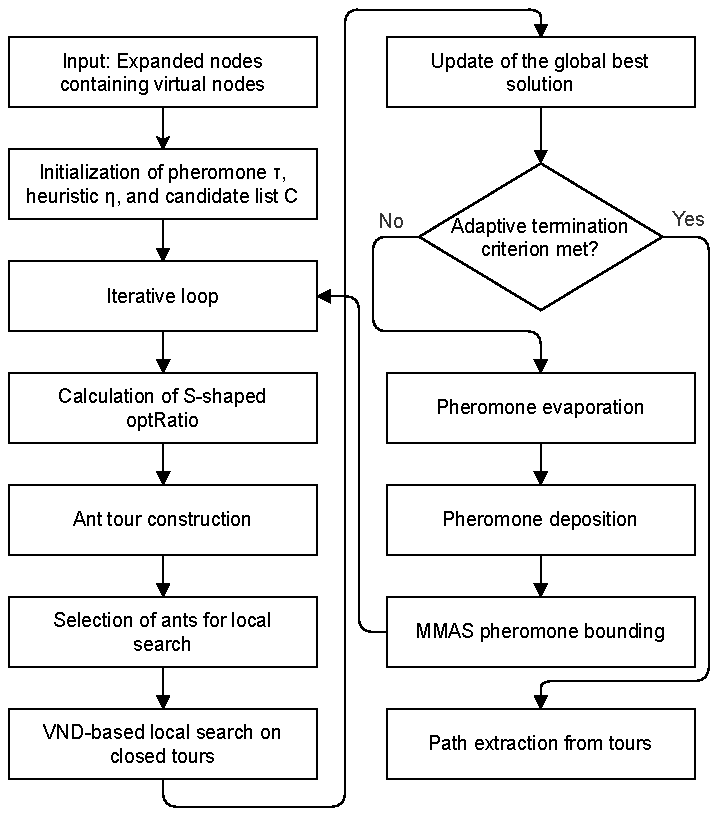
\includegraphics[width=\columnwidth]{figures/fig05_aco_flow.pdf}
\caption{Overall flowchart of the improved ant colony optimization.}
\label{fig:aco_flow}
\end{figure}

\subsection{Cooperative Optimization Framework}
\label{subsec:coop}

The preceding sections have presented the two algorithmic layers separately: the improved A* planner with its post-processing, responsible for point-to-point path finding, and the MMAS-VND-CL solver for the open traveling salesman problem. This section explains how the two are coupled into a complete multi-goal traversal framework.

\subsubsection{Two-Layer Architecture}

The framework is structurally divided into two layers, thereby cleanly separating obstacle-avoiding path finding at the geometric level from visiting-order optimization at the combinatorial level.

The first layer constructs the cost matrix. Given $N$ points consisting of the start point, the end point, and $K$ intermediate goal points, the shortest collision-free path is computed for every pair of points, yielding the pairwise cost matrix $\mathbf{D} \in \mathbb{R}^{N \times N}$. The element $\mathbf{D}(i, j)$ is defined as the length of the shortest collision-free path from point $i$ to point $j$, with diagonal elements set to zero. It should be emphasized that $\mathbf{D}$ is not a Euclidean distance matrix: every element corresponds to the true obstacle-constrained shortest-path length. When obstacles block the straight-line corridor between two points, this length may be substantially larger than the straight-line distance between them.

To make the cost more representative of the robot's actual travel, the path length is not taken directly as the cumulative step count on the grid. Specifically, the grid path obtained from global planning is first simplified in a safety-aware manner, then converted into a continuous trajectory by arc-length-parameterized cubic spline smoothing, and finally $\mathbf{D}(i, j)$ is taken as the sum of Euclidean distances between adjacent sample points along the smoothed trajectory. This both mitigates the staircase effect of grid discretization and better matches the actual motion trajectory. Constructing the complete cost matrix requires $O(N^2)$ calls to the global planner; in practice, a path cache keyed by the start--end coordinate pair may optionally be used to store already-computed pairwise results, avoiding repeated A* searches across multiple traveling salesman solves.

The second layer optimizes the visiting order. It is sufficient to hand the cost matrix $\mathbf{D}$ to the MMAS-VND-CL solver. This layer operates only on a numerical matrix and does not perceive the map, obstacles, or path geometry; all constraint information has been compressed into $\mathbf{D}$. The solver returns the optimal visiting sequence $\bm{\pi}^{*} = (1, \pi_2, \dots, \pi_{K+1}, N)$ and the corresponding total cost $C(\bm{\pi}^{*})$.

\subsubsection{Pipeline Integration}

The complete pipeline can be divided into the following four stages.

\textbf{Point-set assembly.} The $N = K + 2$ points are written into a unified coordinate array $\mathbf{P} = [p_{\mathrm{start}};\; \mathbf{T}_1; \dots; \mathbf{T}_K;\; p_{\mathrm{goal}}]$, with index $1$ designated as the start point and index $N$ as the end point.

\textbf{Cost-matrix construction.} For every ordered pair of points $(i, j)$ ($i \neq j$), the global planner computes the shortest collision-free path from $\mathbf{P}(i,:)$ to $\mathbf{P}(j,:)$, which is written into the path cache; the path is then subjected to safety simplification and spline smoothing, and the Euclidean arc length of the smoothed continuous trajectory is recorded as $\mathbf{D}(i, j)$, making it more consistent with the actual motion trajectory. If no feasible path exists between a pair of points, the corresponding element is set to $\mathbf{D}(i, j) = \infty$. As soon as any goal point is found to be unreachable from the start, the pipeline is aborted immediately and failure is reported.

\textbf{Traveling salesman solve.} The matrix $\mathbf{D}$ and the point count $N$ are handed to MMAS-VND-CL, which returns the optimal visiting sequence $\mathrm{bestOrder} = (1, \dots, N)$ and its total cost. When $K = 0$ (no intermediate goals), the problem degenerates to a trivial case: the sequence is $[1, N]$ and the cost is simply $\mathbf{D}(1, N)$.

\textbf{Output assembly.} The ordered point list $\mathbf{P}(\mathrm{bestOrder}, :)$ is extracted from the coordinate array according to $\mathrm{bestOrder}$, and the individual path segments between consecutive point pairs are retrieved from the path cache and concatenated into the final obstacle-free reference path set.

\subsubsection{Design Rationale}

Separating the two layers offers three main advantages.

First, the planner and the traveling salesman solver can be developed, tested, and improved independently. The first layer can be replaced by any grid-based planner (A*, Dijkstra, RRT, etc.), and the second layer by any permutation optimization algorithm (ant colony optimization, genetic algorithm, simulated annealing, etc.). This modular design is validated in the experiments of Sections~\textcolor{blue}{\ref{subsec:exp_sens}}--\textcolor{blue}{\ref{subsec:exp_cmp}}: when alternative implementations of one layer are compared, the other layer is kept unchanged.

Second, the cost matrix $\mathbf{D}$ serves as a compact interface. Regardless of environmental complexity, the $N \times N$ matrix completely records the obstacle-constrained distance relationships among all point pairs. The traveling salesman solver therefore does not need access to the grid map, yet still enjoys feasibility guarantees in the obstacle-avoidance sense. Of course, this compression entails some information loss: the solver cannot determine whether two path segments share the same narrow corridor. But for the objective of ``minimizing total cost'', the representation is sufficient.

Third, using the Euclidean arc length of the smoothed continuous trajectory as the pairwise cost makes the distance measure on which the combinatorial optimization is based closer to the actual motion trajectory. If the raw grid path were measured by accumulating orthogonal and diagonal steps, the staircase polyline would systematically overestimate the continuous travel distance; after safety simplification and spline smoothing, the cost matrix more closely approximates the path length actually tracked by the robot, providing the traveling salesman solver with a more execution-faithful distance basis for comparing different visiting orders.

\subsubsection{Complete System Flow}

In end-to-end execution, the system completes the following steps in sequence:
\begin{enumerate}
\item \textbf{Construct the cost matrix}: call the improved A* planner for all $O(N^2)$ point pairs and evaluate the resulting paths after safety simplification.
\item \textbf{Solve the open traveling salesman problem}: call MMAS-VND-CL to determine the optimal visiting sequence.
\item \textbf{Retrieve the individual path segments}: concatenate the complete trajectory from the path cache according to the visiting sequence.
\item \textbf{Post-processing}: apply path simplification and cubic spline smoothing to each segment, outputting smooth obstacle-free continuous trajectories.
\end{enumerate}
The overall system architecture is shown in Fig.~\textcolor{blue}{\ref{fig:system}}.

\begin{figure}[!htbp]
\centering
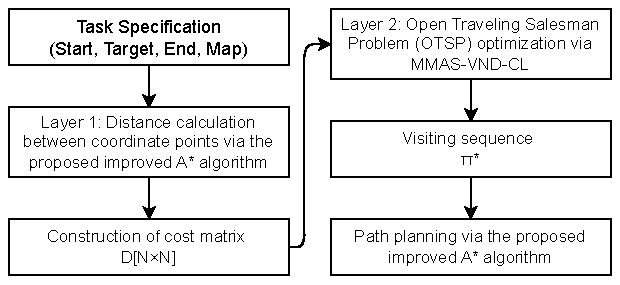
\includegraphics[width=\columnwidth]{figures/fig06_system.pdf}
\caption{Overall system architecture.}
\label{fig:system}
\end{figure}
